\begin{exerciseS}[Vortice lineare nel piano]
 Utilizzando l'espressione dela velocità indotta da un vortice irrotazionale puntiforme di intensità unitaria,
\begin{equation}
 \bm{u} = \dfrac{1}{2\pi r} \bm{\hat{\theta}} \ ,
\end{equation}
 dimostrare che la velocità indotta nel punto $\bm{P}$ da un vortice di intensità unitaria uniforme distribuito sul segmento che congiunge i due punti $\bm{N}_1$, $\bm{N}_2$ vale
\begin{equation}
 \bm{u} = - \dfrac{1}{2\pi} \beta \bm{\hat{x}} 
 - \dfrac{1}{2\pi} \ln \dfrac{|\bm{r}_2|}{|\bm{r}_1|} \bm{\hat{y}} \ ,
\end{equation}
 essendo $\bm{\hat{x}}$, $\bm{\hat{y}}$ i versori in direzione tangente e normale al segmento $\bm{N}_1 \bm{N}_2$, i vettori $\bm{r}_i = \bm{P} - \bm{N}_i$, $i = 1:2$ e $\beta$ l'angolo compreso tra il vettore $\bm{r}_1$ e il vettore $\bm{r}_2$, positivo se si deve ruotare il vettore $\bm{r}_1$ in senso antiorario per farlo coincidere con $\bm{r}_2$.
\end{exerciseS}

\begin{center}
\begin{figure}[h]
\centering
\includegraphics[width=0.40\textwidth]{./fig/pointVortex}
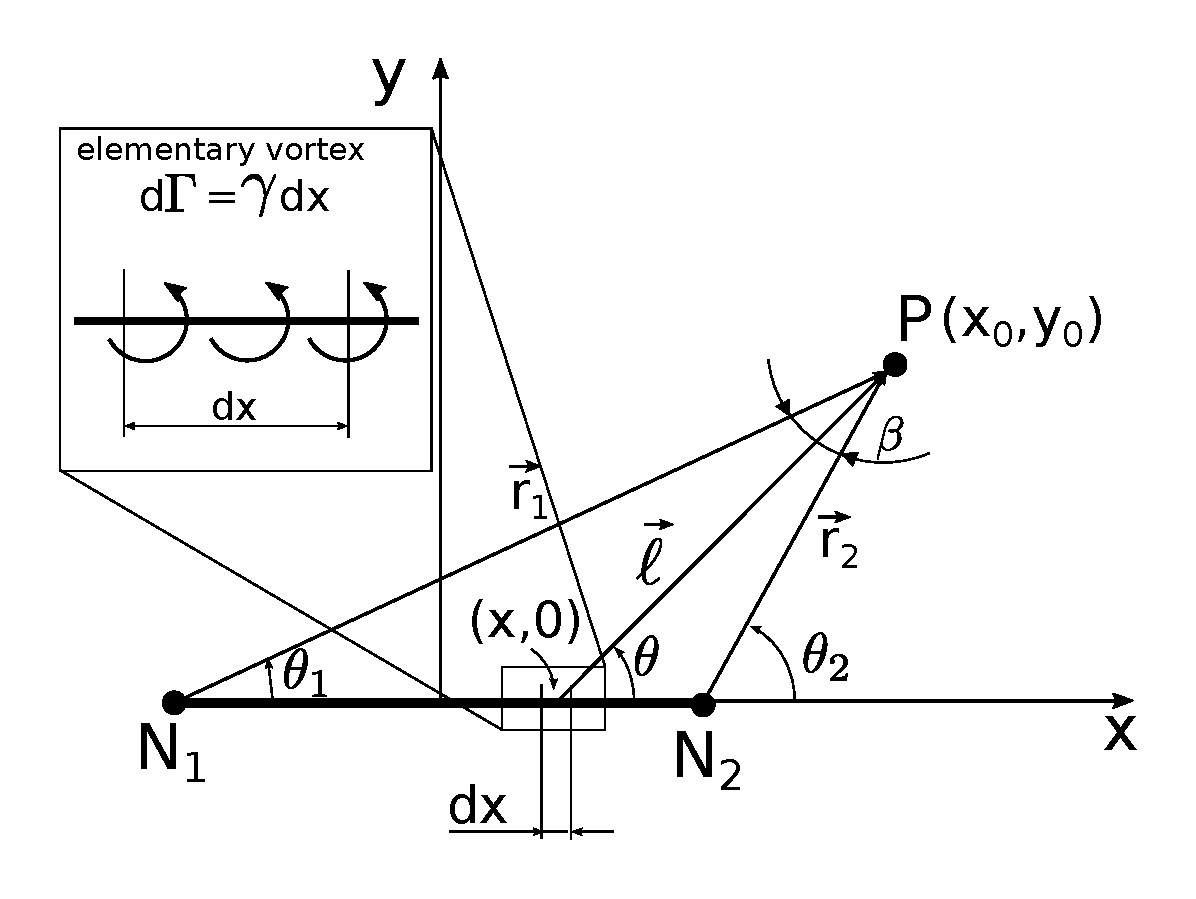
\includegraphics[width=0.50\textwidth]{./fig/lineVortex}
\caption{Rappresentazione di un vortice irrotazionale puntiforme e del vortice distribuita sul segmento $\bm{N}_1 \bm{N}_2$: definizione della ``densità lineare di vortice'' $\gamma$ e delle quantità geometriche.}\label{fig:lineVortex}
\end{figure}
\end{center}
